\chapter{Forschungsstand}
\label{ch3:Forschungsstand}

\section{Gamification}
\label{ch3:s:Gamification}

Der Begriff Gamification geht auf Nick Pelling im Jahr 2002 zurück.\cite{Pelling.2011}
Er beschreibt den Prozess, bei dem Spielmechaniken auf bestehende Aspekte angewendet werden, um eine extrinsische Motivation zu erzeugen.\cite{Marczewski.2013}
Erste Gamification Ansätze gab es zu Beginn des 20. Jahrhunderts z.\,B. durch Stempelkarten an der Eisdiele. Später wurden ähnliche Konzepte in Vielfliegerprogrammen aufgegriffen.

In der Literatur gibt es unterschiedliche Definitionen der Gamification.
In der nachfolgenden Tabelle \ref{table:ch3:lit_overview} sind verschiedene Autoren und deren Einordnung des Gamification Begriffs zu sehen.
Es lässt sich zunächst feststellen, dass ein gemeinsamer Konsens in der Literatur darüber herrscht, dass Gamification eine Nutzung von Spielmechaniken darstellt.
Beim Vergleich der Einzelnen ist erkennbar, dass \textcite{Zichermann.2011} und \textcite{Kapp.2012} eine Übereinstimmung in der Nutzung von Gamification als Motivation finden. Zudem findet eine Überschneidung bei der Verwendung von Gamification als Mittel zur Lösung von Problemen statt. \textcite{Zichermann.2011} definieren hier die Gamification als Mittel um extrinsische Motivation zu erzeugen, welche entsprechend Einfluss auf die Handlungen des Einzelnen hat.
\textcite{Deterding.2011}, \textcite{Breuer.2011} und \textcite{Oxford.2013} grenzen im Vergleich dazu die Gamification von normalen Spielen explizit ab. Sie legen Wert darauf, dass keine Spiele als Gamification verstanden werden, sondern als Basis der Gamification eine normale spielfremde Tätigkeit steht.
\textcite{Kapp.2012} geht im Vergleich zu den restlichen Autoren hier weiter und ergänzt die Nutzung von Gamification als Lehrmittel und stellt diese als Motivation für Personen dar. Speziell die Nutzung von Gamification im Zusammenhang der Lehre lässt sich in der aktuellen Literatur ebenfalls verfolgen.\cite{Loh.2012}
Nach \textcite{Jeannerod.2003} kann Gamification genutzt werden um ein Empowerment der partizipierenden Spieler zu erreichen.
Ein Beispiel für die Nutzung von Gamification stellt das Sammeln von Geoinformationen mithilfe einer App dar.\citep{Odobasic.2013}

%%\begin{table}
\begin{sidewaystable}
\footnotesize
\begin{tabular}{|l|l|l|l|l|l|}
\hline
~ & \textcite{Zichermann.2011} & \textcite{Deterding.2011} & \textcite{Breuer.2011} & \textcite{Oxford.2013} & \textcite{Kapp.2012} \\
\hline\hline 
Nutzung von Spielmechanik & X & X & X & X & X \\
\hline
Motivation & X & ~ & ~ & ~ & X \\
\hline
Problemlösung & X & ~ & ~ & ~ & X \\
\hline
Spielferner Kontext & ~ & X & X & X & ~ \\
\hline
Verhaltensbeinflussung & ~ & ~ & X & ~ & ~ \\
\hline
Lernförderung & ~ & ~ & ~ & ~ & X \\
\hline
Anregung zum Handeln & ~ & ~ & ~ & ~ & X \\
\hline
\end{tabular}
\label{table:ch3:lit_overview}
\caption{Literaturübersicht zur Definition von Gamification}
%%\end{table}
\end{sidewaystable}



\begin{figure}[H]
\begin{center}
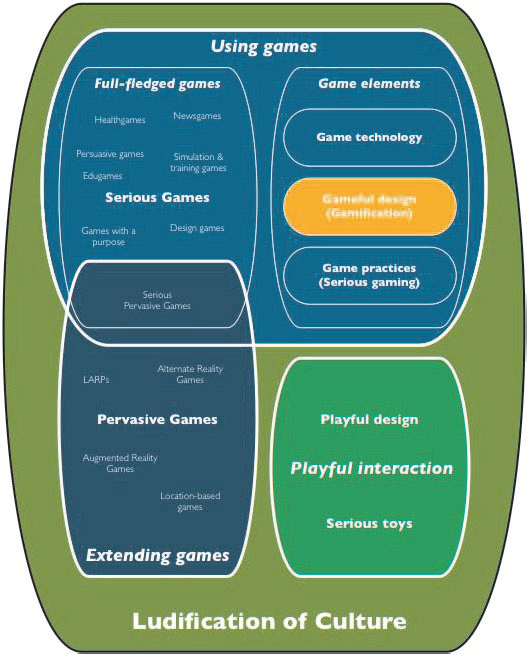
\includegraphics[width=100mm]{images/ch3_img02_gamification.png}
\caption{Gamification nach \textcite{Deterding.2011}}
\label{img:ch3_img02_gamification}
\end{center}
\end{figure}

Eine Einordnung und Abgrenzung der Terminologie ist in \ref{img:ch3_img02_gamification} zu sehen. \textcite{Deterding.2011} grenzen hierbei die Gamification als Prozess ab, der für die Erstellung der Spielelemente dient. Dieser Prozess wird verwendet um unter anderem Serious Games erstellen zu können. Diese stehen wiederum im Kontrast zu den Spielen zur normalen Unterhaltung, welche als Ausgangsbasis keinen alltäglichen Sachverhalt besitzen.

In der Literatur werden die Elemente Points, Badges und Leaderboards (PBL) angesprochen. Diese dienen als Mittel um eine Gamification durchführen zu können. 
Points stellen Punkte dar, die verwendet werden um einen Fortschritt des einzelnen Spielers darzustellen. Dies sind zum Beispiel Meilen in Vielfliegerprogrammen oder Statuspunkte beim Bonus Programm der Deutschen Bahn.

Bei Badges handelt es sich um Abzeichen, welche für bestimmte Errungenschaften an den Spieler vergeben werden. Ein Beispiel hierfür ist das Trainspotter Badge bei Foursquare, welches ausgestellt wird, wenn der Spieler in eine gewisse Anzahl von Bahnhöfen besucht hat. Die Badges sollen einen gewissen Status gegenüber den restlichen Spielern suggerieren.

Leaderboards sind klassische Ranglisten. Diese dienen dazu einen Wettbewerb unter den Spielern zu erzeugen. Hierbei wird empfohlen nicht auf die klassische Top10 Liste zurückzugreifen, wie es bei vielen Spielhallen Automaten üblich ist. Stattdessen soll der Spieler zwischen Anderen platziert werden. Hierbei sind im Idealfall die Ränge über und unter dem Spieler dessen Freunde (vgl. Foursquare). Dies verhindert, dass der Spieler von überhöhten Punktzahlen abgeschreckt wird.

\textcite{Zichermann.2011} erweitern das Modell in dem Sie es um weitere Aspekte ergänzen und diesem Struktur verleihen.
Sie verwenden den Begriff SAPS. Dieser unterteilt sich in Status, Access, Power und Stuff (SAPS).
Das bekannte Points, Badges und Leaderboards der Literatur wird unter Status zusammengefasst wie in nachfolgender Aufzählung zu sehen.

\begin{itemize}
\item Status (Badges, Levels, Leaderboards)
\item Access (early Access)
\item Power (give power, e.g. modicum control over other players)
\item Stuff (give a reward, try to prevent that the price gets known)
\end{itemize}

Bei Access handelt es sich um \glqq Zugriff\grqq{} zu exklusiven Dingen, welche man dem Spieler gewährt. Ein Beispiel hier für ist die Lufthansa Senator Lounge oder die DB Lounge.
Es kann sich aber auch um einen zeitlich verfrühten Zugriff auf ein Produkt oder Funktionen handeln.

Unter Power sind Regeln zu verstehen, welche es dem Spieler erlauben Einfluss (Macht) auf andere Spieler auszuüben. Dies kann z.\,B. durch Moderationsrechte ab einem bestimmten Level realisiert werden. Foursquare realisiert dies durch Superuser.\cite{Lindqvist.2011}

Der letzte Punkt stellt Stuff dar. Hierbei handelt es sich um Belohnungen die dem Spieler zuteilwerden. Klassischerweise handelte es sich hierbei z.\,B. um ein zusätzliches kostenloses Eis. Ziel ist es, dass dem Spieler nicht der konkrete monetäre Gegenwert ersichtlich wird. D.h. der Spieler soll nicht erkennen, wie viel seine Belohnung wert ist. Das Ziel sollte es nicht sein dem Spieler kostenlose Produkte zu geben, sondern etwas, was seinen Status unterstreicht.\\

Im Zuge der Gamification wird gerne der Begriff des Flow-Zustandes aufgegriffen.
Hierbei handelt es sich um einen von \textcite{Csikszentmihalyi.1991} eingeführten Begriff, bei dem es darum geht den Spieler zwischen einem optimalen Zustand zwischen Anspannung und Langeweile zu halten. Im Flow Modell wird angenommen, dass der Mensch sich in einer Situation jeweils seiner Handlungsmöglichkeiten und Fähigkeiten bewusst ist.
Übersteigt der Umfang der Aufgaben die Fähigkeiten, stellt sich ein Zustand oberhalb des Flow-Zustandes ein, wie in Abbildung \ref{img:ch03_img02_flow} zu sehen. Bei einer Unterforderung oder Einschränkung der Handlungsmöglichkeiten stellt sich schnell Langeweile ein. Das Ziel ist es den optimalen Zustand für den Spieler zu finden. Viele Spiele arbeiten unter anderem mit dynamischen Schwierigkeitsstufen, die berüchtigte Gummi-Band KI ist ein klassisches Beispiel.\cite{Bateman.2011}

\begin{figure}[H]
\begin{center}
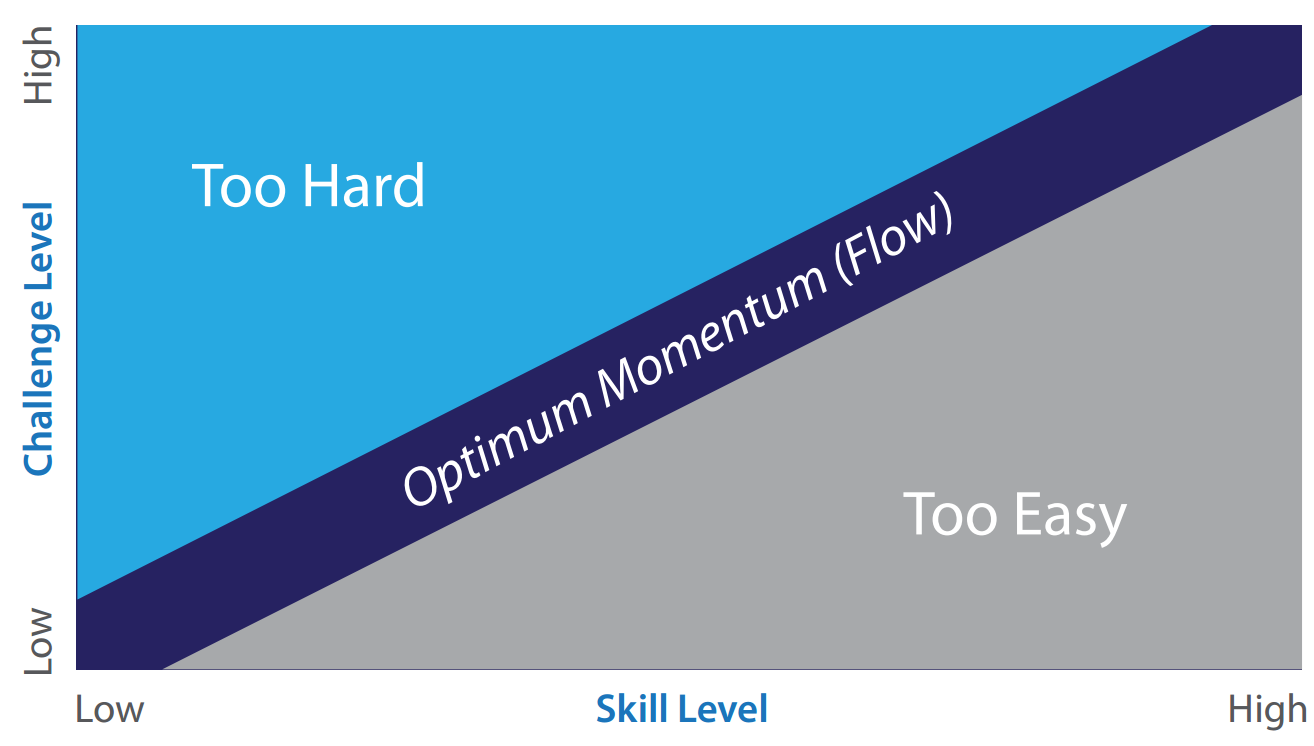
\includegraphics[width=120mm]{images/ch03_img02_flow.png}
\caption{Flow Zustand nach \textcite{Csikszentmihalyi.1991}}
\label{img:ch03_img02_flow}
\end{center}
\end{figure}

\section{Location-based Games}
\label{ch3:s:Geogames}

\subsection*{Spiel}

Für die Definition von Geogames, muss zunächst der Spiel-Begriff definiert werden. In der Literatur gibt es hierfür eine Vielzahl von Definitionen.
In dieser Arbeit soll die Definition analog zu \textcite{Salen.2010} verwendet werden, welche ein Spiel als Situation in Abgrenzung zum normalen Alltag darstellen. Ein Spiel wird innerhalb eines sogenannten Magic Circles durchgeführt, welcher das Spiel und die teilnehmenden Spieler von der Realität abgrenzt.
Dieser magische Kreis dient als Regelraum in welchem dann ein Spiel nach vorgegebenen Regeln durchgeführt wird. Im Kontrast stehen hier zu Alltagssituationen, wie das Einkaufen oder die Arbeit.

%\subsection*{Spielertypen}

\subsection*{Mobilegames}

Unter Mobilegames sind Spiele aller Art zu verstehen, die unterwegs gespielt werden. Diese werden auf mobilen Endgeräten gespielt.\cite{Bell.2006} Unter Mobile Endgeräte fallen klassische Handheld-Konsolen wie z.\,B. der Nintendo Game Boy und Smartphones.

\subsection*{Location-based Games}

Ortsbezogene Spiele werden in einem Geokontext gespielt werden. Hierbei wird die aktuelle Position des Spielers als Kontrollelement verwendet.\cite{Schlieder.2006} Durch dieses kann der Spieler mit dem Spiel interagieren.
Geogames sind eine Spezialisierung von ortsbezogenen Spielen, welche als Ursprung meist ein Brettspiel haben.
Geogames sind nicht begrenzt auf digitale Spiele, sondern haben Ihren Ursprung im Versteckspiel, auch in Form einer Schnitzeljagd. Ein späterer Nachfolger dieser stellt das Geocaching dar.\cite{Simanowski.2008}
Das Ziel der ortsbezogenen Spielen ist die Interaktion des Spielers mit der Umgebung. Dies unterscheidet sich von den klassischen Konsolen-Spielen, bei denen der Spieler das Spielgeschehen über einen Controller steuert. Grenzt man diese motorische Steuerung ab, gibt es die Zwischenstufe des Vistaspaces. Im Vistaspace steuert der Spieler das Spiel nicht mehr mit seinen Händen, sondern mit motorischen Bewegungen. Beispiele hierfür sind die Nintendo Wii und die Xbox Kinect. Bei diesen werden durch Lagesensoren und Infrarot Kameras die Bewegungen des Spielers erfasst und in die Spielsituationen eingebunden.
Findet das Spiel außerhalb eines Raumes statt, so wird vom sogenannten environmental space gesprochen.
Hierbei findet die Steuerung der Spiels und somit der Spielerposition durch Lokomotion statt.\cite{Benford.2003,Kiefer.2007}
Die drei kognitiven Räume beschreibt \textcite{Berendt.1999} in einer Gegenüberstellung der einzelnen Attribute.
\\\\
In der aktuellen Literatur werden vermehrt Spiele für Smartphones untersucht und entwickelt.\cite{Rashid.2006a}
Durch die Integration von GPS-Modulen, den fallenden Preisen für die mobile Datenübertragung und der Vereinfachung der Entwicklung entsprechender Spiele stehen diesen einer wachsenden Zielgruppe gegenüber.
\\\\
Eine Spezifizierung der ortsbezogenen Spiele stellen die sogenannten Geogames dar. Dieser Begriff wird vor allem von \textcite{Schlieder.2013} gepflegt. Hierbei handelt es sich überwiegend um klassische Brettspiele, deren Spielkonzept auf ortsbezogene Spiele übertragen wird. Die Grundidee ist es, die strategischen Reize der Brettspiele mit den Affordanzen der Echtzeit Situation von ortsbezogenen Spielen zu verbinden. Dabei wird die rundenbasierte Spielmechanik ausgetauscht gegen die Lokomotion des Spielers. Die damit verbundenen Probleme und Schwierigkeiten werden in \textcite{Schlieder.2006} beschrieben.

\subsection*{Pervasive Games}

Unter Pervasive Games sind Spiele zu verstehen, welche den Magic Circle in seinen abgrenzenden Dimensionen erweitern.
Konkret werden die definierten Grenzen typischer Spiele überschritten.\cite{Montola.2005}
Hierbei geht es um die Erweiterung der ortsspezifischen, zeitlichen und sozialen Grenzen.\cite{Montola.2009}
Darüberhinaus gibt es in der Literatur bei \textcite{Nieuwdorp.2007} und \textcite{Bjork.2007} eine weitere Dimension, welche als \glqq ambiguity 
of interaction or interface\grqq{} definiert wird. Hierbei handelt es sich um die Unklarheit bzw. Eindeutigkeit der Interaktion.
Eine Vielzahl von Pervasive Games wurde in der Literatur behandelt und die Spielerinteraktion entsprechend untersucht.
Beispiele hierfür sind Can You See Me Now \cite{Flintham.2003}, GeoTicTacToe, CityPoker, Neocartographer von \textcite{Schlieder.2005}, Human Pacman \cite{Cheok.2003} und Feed my Yoshi \cite{Bell.2006}.
Anhand dieser Spieler wurden Erkenntnisse in der Praxis gewonnen, welche sich mit der Gamification Literatur in Kapitel \ref{ch3:s:Gamification} decken.
Eine Sammlung weiterer interessanter Spielkonzepte stellt die Sammlung von \textcite{Hinske.2007} dar, welche Ideen für eigene Spielideen liefern kann.
Für die Umsetzung des Frameworks ist es wichtig einen Überblick und Einordnung über die aktuell existierenden Pervasive Games zu haben. Aufgrund dieser Informationen können bewusst bessere Entscheidungen im Entwurf getroffen werden, welche somit dem Spielleiter und dem darauf aufbauenden Spiel zugute kommen.


\section{Relokalisierungsansätze}
\label{ch3:s:Relokalisierung}

Ein wichtiger Aspekt im Zuge von Pervasive Games ist der Gamecontent. Soll ein Spiel außerhalb eines fest definierten Geografischen Raums durchgeführt werden, ist es notwendig entsprechende fremde Umgebungen mit Inhalt zu füllen.\cite{Montola.2005} 
Bei der ortsbezogenen Relokation von Spielinhalten gibt es unterschiedliche Ansätze.
Zunächst müssen die ortsbezogenen Affordanzen beachtet werden. Hierbei handelt es sich um die lokalen Gegebenheiten, welche einen Einfluss auf das Spielgeschehen haben. Ein Beispiel hierfür sind Flüsse die ein Spielfeld teilen und damit die Distanz zwischen zwei einzelnen Spielelementen beeinflussen.
\\\\
Es gibt in der Literatur einen ersten Ansatz für die Relokalisierbarkeit von Spielfeldern.
\textcite{Kiefer.2005} beschreiben die Überlegungen bei der Durchführung des GeoTicTacToe Spiels in Bamberg. Bei der die Anordnung der 9 Spielpunkte einen Einfluss auf das Spielgeschehen hat. Brücken, Gebäude und Wege sind nicht strikt linear oder in Quadraten wie in vielen amerikanischen Städten oder z.\,B. in der Mannheimer Innenstadt. Für eine perfekte Ausgeglichenheit der Spielfelder müssten jegliche Informationen über Entfernungen, Fußgängerampeln Steigung des Wegs, körperliche Verfassung des jeweiligen Spielers, sowie dessen spatiale Fähigkeiten vorhanden. Dadurch entsteht ein äußerst komplexes Modell ohne Ideale Lösung. Daher wurden die ortsbezogenen Affordanzen als gegeben hingenommen bzw. in das Spiel als Herausforderung bzw. Spielelement integriert.

Generell gibt es drei Ansätze zur Relokation der Spielemente auf einer Karte.

\begin{itemize}
\item Keine Anpassung -- Spiel an einem Ort möglich
\item Komplette Anpassung -- Spiel an jedem Ort möglich
\item Hybride/teilweise Anpassung -- Spiel durch Eingriffe spielbar
\end{itemize}

In der Literatur werden die Probleme von ortsbezogenen Spielen öfters angesprochen, jedoch keine konkreten Lösungsansätze untersucht.
Die erste Möglichkeit stellen Spiele dar, welche keinerlei Anpassung enthalten.
Ein Beispiel hierfür ist REXplorer.\cite{Ballagas.2007} REXplorer ist nur in der Stadt Regensburg spielbar. Neben dem zugeschnittenen Geolocation Content ist der Controller explizit auf die Umgebung angepasst.
Hierbei handelt es sich um eine Art Zauberstab mit dem der Spieler mit den Elementen in der Umgebung interagieren kann. Diese Elemente sind jedoch explizit nur für die Stadt Regensburg erstellt worden und somit ist eine Funktion außerhalb nicht möglich.

Im Gegensatz dazu steht die zweite Möglichkeit. Hierbei handelt es sich um Spiele, welche komplett ortsunabhängig gespielt werden können.
Dies kann entweder durch einen Algorithmus sicher gestellt werden oder durch die Tatsache, dass die Spielelemente keinen direkte Anpassung benötigen.
Spiele wie Feed my Yoshi, welche keine direkte Anpassung benötigen, haben deutliche Unterschiede im Hinblick ihrer Spielbarkeit abhängig von ihrer Umgebung. Die Autoren stellten  eine Korrelation zwischen Bevölkerungsdichte und Spielbarkeit fest, da die Spielelemente von WLAN-Accessspoints generiert wurden.\cite{Bell.2006}

Die letzte Möglichkeit stellt ein hybrider Ansatz dar. Bei diesem werden bestehende Spielfelder von einem vorgegebenen geografischen Kontext auf ein anderes Spielfeld übertragen. Hierbei wird unter Zuhilfenahme von Algorithmen ein Transfer der bestehenden Daten auf ein neues Spielfeld bewerkstelligt.
\\\\
Konkrete Lösungsansätze sind in der Literatur mit der Ausnahme von \textcite{Kiefer.2007}
nicht zu finden.
Der von \textcite{Kiefer.2007} gewählte Ansatz zielt darauf ab ein Vergleich von verschiedenen Spielfeldern herzustellen um Spieler von verschiedener Herkunft gegeneinander antreten können. Ziel ist es den Aufwand und die Kosten für die Durchführung dieser Spiele zu reduzieren. \textcite{Kiefer.2007} identifiziert drei Quellen die zu einer Heterogenität der Spielfelder führen:

\begin{itemize}
\item spatial scale -- Unterschied in geografische Größe
\item static structure -- Unterschied in geografischer Struktur (Straßen, Höhe) 
\item dynamic conditions -- Verändernde Gegebenheiten (Wetter, GPS/GSM-Empfang, Verkehr)
\end{itemize}

Eine gewisse Heterogenität der Spielfelder macht die Herausforderung für die Spieler interessanter. Zu große Unterschiede führen hingegen zu einem unfairen und damit weniger gutem Spielerlebnis.
Generell gibt es zwei Arten von ortsbezogenen Spielen. Zum einen örtlich begrenzte (spatial discrete) Spiele und zum anderen örtlich fortsetzende (spatial
continuous) Spiele.
Bei Ersterem handelt es sich um Spiele die auf einem abgegrenzte Spielfeld durchgeführt werden und die Position des Geocontents fest auf der Karte definiert ist. Letztere sind Spielfelder, welche unbegrenzte Spielfelder haben und die Spielinteraktion zu jeder Position stattfinden kann.
Im Falle der spatial continuous Spiele ist ein bijectives Mapping der Orte nötig.
Bei einer Bijektion findet eine vollständige Paarbildung zwischen den Elementen von Ursprungsspielfeld und Zielspielfeld statt.\cite{Athanasiadis.1999}
Dies funktioniert gut bei offenen Flächen. Bei der Verwendung von Straßen und innerhalb von Städten führt dies zu einer starken Verzerrung der Spielfelder und zu einem Diskrepanz zwischen Spielerfortbewegung und Lokomotion im Spiel.
Dies war der Grund, dass \textcite{Kiefer.2005b} spatial discrete Spiele im Detail untersucht haben.
Konkret wurde das Spiel CityPoker\cite{Kiefer.2005b} in zwei verschiedenen Städten gleichzeitig gespielt. Dabei konnten beide Teams der jeweiligen Städte über vordefinierte POIs miteinander interagieren. Untersucht wurde die optimale Gestaltung der Spielfelder, damit diese zwischen den Städten den kleinsten Unterschied zueinander darstellen. Zunächst wurden die POIs für beide Städte manuell nach eigenem Ermessen ausgewählt. Im Anschluss auf die Spielsitzung wurde untersucht, wie die unterschiedlichen Spielfelder ausgewählt werden müssten um ein optimales Feld zu erhalten. Hierbei ist zu beachten, dass die Reihenfolge der POIs bei Citypoker eine Rolle spielt.
Abbildung \ref{img:ch3_img03b_distributed} beschreibt ein ausgewähltes Spielfeld, sowie Distanzen zwischen den einzelnen Punkten.
Am Punkt 1 können Karten getauscht werden, welche beim anderen Team ebenfalls auf 1 liegen. \cite{Kiefer.2007} stellt für den Vergleich eine Entfernungsmatrix auf, welche über ein Ähnlichkeitsmaß gegenüber gestellt werden.
Für die Berechnung der Ähnlichkeit wird nachfolgendes Maß angewandt:

\begin{equation}
similarity = \frac{1}{n} \sum_{row=1}^{n} \sqrt{ \sum_{col=1}^{n} (c_{1,row,col} - c_{2,row,col})^2 }
\end{equation}

Hierbei stellen $c_1$ und $c_2$ jeweils die Entfernungsmatrizen der jeweiligen Spielfelder dar.
Row und col adressieren hierbei die Zeile und Spalte.
Zu beachten ist, dass die Entfernungen als direkte euklidische Luftlinie gemessen werden. Etwaige Höhenunterschiede, sowie örtliche Gegebenheiten werden hierbei aus Gründen der Vereinfachung nicht beachtet. Anschließend wird das arithmetische Mittel der Durchschnittswerte der einzelnen Reihen gebildet.
Als Ergebnis wird angenommen, dass spatial discrete Spiele eine einfachere Konfiguration erlauben wie unter anderem \textcite{Benford.2005} angemerkt hat.

\begin{figure}[H]
\begin{center}
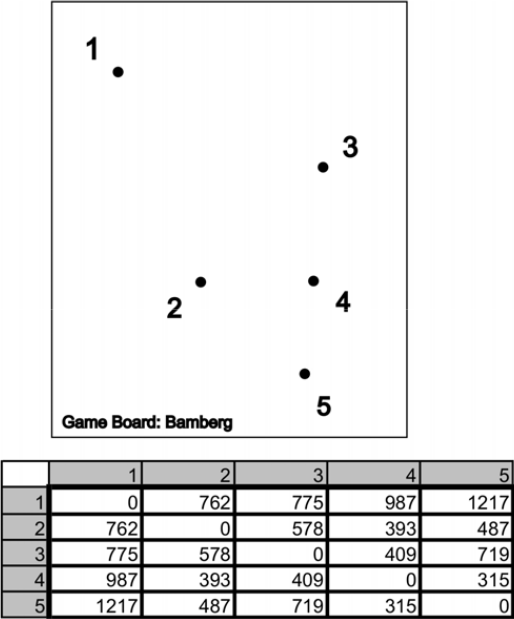
\includegraphics[width=100mm]{images/ch3_img03b_distributed.png}
\caption{Spielfeld Verteilung nach \textcite{Kiefer.2007}}
\label{img:ch3_img03b_distributed}
\end{center}
\end{figure}

\textcite{Benford.2005} identifizieren mehrere Herausforderungen im Bezug auf spatial continous games.

\begin{itemize}
\item Hefting domains
\item Configuration
\item Orchestration
\end{itemize}

Hefting domains stellen die Problematik dar, dass Spielelemente in Computerspielen auf die virtuellen Spielwelt fokussiert sind. Bei Pervasive Games muss dagegen ein besonderer Wert auf die Designentscheidungen bezüglich der virtuellen, reellen und hybriden Spielelemente gelegt werden.

Unter der Configuration ist die Adaption von Pervasive Games an verschiedene lokale Gegebenheiten zu sehen, d.h. die (generierte) Erstellung von Spielfeldern an anderen Orten.

Die Orchestration stellt das Management des Spiels während der Laufzeit dar. Hierbei soll sichergestellt werden, dass ein Eingriff in das Spielgeschehen zu Gunsten der Sicherheit der Spieler als des Spielerlebnisses möglich ist.

Ein erster Ansatz für die automatisierte Relokalisierung von Spielfelder lässt sich in der Literatur bei \textcite{Mannara.2012} finden. Dieser entwirft eine DSL\footnote{domain-specific language} zur Nutzung von OSM Daten für das Auffinden von Spielelemente des gleichen Typs am Beispiel von Uni Campi.
\\\\
Abschließend lässt sich feststellen, dass in der Literatur keine konkrete Lösung für die (teil-)automatisierte Erstellung von Spielfeldern existiert.
An dieser Stelle soll die Arbeit des Autors ansetzten und eine Lösungsmöglichkeit präsentieren.
Die daraus gewonnen Erkenntnisse sollen eine weitere Diskussion der Thematik ermöglichen.

\section{Verwendung offener Geodaten}
\label{ch3:s:offeneGeodaten}

Zunächst ist der Begriff offene (Geo-)Daten zu definieren.
Unter offenen Daten sind im folgenden Daten zu verstehen, welche unter freier Lizenz zur Verfügung stehen und somit ohne Lizenzgebühren verwendet werden können. Hierbei soll im Idealfall sowohl eine kommerzielle Nutzung als eine private Verwendung erfolgen können.
Es lassen sich generell zwei verschiedene Quellen von öffentlichen Geodaten identifizieren.
Als erste Möglichkeit sind es Daten von öffentlichen Behörden. Hierbei gibt es aktuell im Zuge der Open Data Bewegung \cite{Oreilly.2007} den Anspruch Daten diverser Behörden den Bürgern zur Verfügung zu stellen. Der Grund liegt in der Argumentation, dass diese Daten mit Hilfe von Steuergeldern erstellt wurden. Erste Ansätze lassen sich sowohl in Großstädten wie Wien \cite{Wien.2014}, Hamburg \cite{Hamburg.2014} und Berlin \cite{Berlin.2014} finden. Als Beispiel für ganze Länder ist Dänemark \cite{Denmark.2014} zu nennen.\footnote{Eine Übersicht ist unter \url{http://www.engagedata.eu/opendatasites} (Abgerufen am 11.02.2014) zu finden. } Die Art, Qualität, sowie Umfang der Daten unterscheiden sich . 
Die zweite Option sind offene (Geo-)Datenbanken, welche von privaten Personen durch manuelles Mapping oder externe lizenzierte Quellen zusammen getragen werden.
Beispiele entsprechender Datenbanken sind OpenStreetMap (OSM)\footnote{\url{http://OpenStreetMap.org}} und Wikimapia\footnote{\url{http://wikimapia.org}}.
Hierbei stellt sich vor allem die Frage der Qualität der Daten im Vergleich zu kommerziellen bzw. Daten von Behörden.

\begin{figure}[H]
\begin{center}
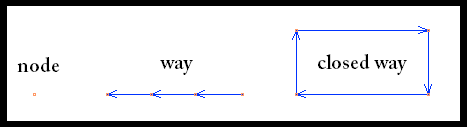
\includegraphics[width=120mm]{images/ch3_img03_OSM1.png}
\caption{OSM Elemente}
\label{img:ch03_img03_OSM1}
\end{center}
\end{figure}

Da für die Umsetzung des Frameworks OSM zum Einsatz kommen soll, ist eine Einschätzung im Hinblick auf die Anforderungen notwendig.
In Abbildung \ref{img:ch03_img03_OSM1} sind ein Teil der Standard Elemente von OSM zu sehen.
Generell werden alle Kartendaten durch Nodes, Ways und Relations dargestellt. Ways sind miteinander verbundene Nodes und Relations enthalten Relations, Ways, Nodes.
Für jeder der drei Typen können entsprechende Tags definiert werden. Damit können jedem Objekt mehrere Key-Value paare zugewiesen werden, welche als Attribute zur Beschreibung der Objekte dienen.

In der Literatur haben sich viele Autoren mit der Qualität von OSM beschäftigt.
\textcite{Haklay.2010}, \textcite{Flanagin.2008} und \textcite{Goodchild.2007} beschreiben die Motivation der Personen die Kartenmaterial pflegen. Darüber hinaus wird auf die Probleme in offenen Datenbanken eingegangen. Es wird angemerkt, dass je nach Ziel des Mappers eine unterschiedliche Qualitätsstufe erreicht wird.
\textcite{Girres.2010} beschreiben in einem Vergleich von französischer Daten, dass die Qualität der Daten von OSM seit dem Start 2004 deutlich zugenommen hat. Auf dem Land gibt es im Vergleich zu Städten unterschiedliche Abdeckungsraten. Zudem haben Naturkatastrophen einen Einfluss auf die Qualität der Daten.\cite{Zook.2010}
Zur Zeit gibt es bei OSM ca. 25.000 aktive Mapper \cite{OSM.2013}. Die Autoren stellen eine Korrelation zwischen Einwohnerdichte und Datenqualität fest.
Die durchschnittliche Abweichung der Position beim Vergleich von OSM zu kommerziellen Kartenherstellern beträgt zwischen 1 und 30 Metern.
Darüber hinaus gibt es eine Ungenauigkeit bei Namen von Objekten. Diese entstehen unter anderem durch die Nutzung unterschiedlicher Sprachen und durch lokale Besonderheiten.
Die Einfachheit von OSM durch die Reduktion der Daten auf Nodes, Ways und Relations mit den dazugehörigen Tags hat den Nachteil, dass im Modell keine logische Konsistenz sichergestellt wird. Dies muss in der Verarbeitung der Daten berücksichtigt werden.
\textcite{Hecht.2013} beschreibt, dass eine geringe Abdeckungsrate im Vergleich zu professionellen Daten gibt. Dies wird ebenfalls von \textcite{Pfoser.2013} angemerkt. Dieser weist allerdings darauf hing, dass OSM eine hohe Klassifikationsrate besitzt. Zwar stellt der Autor eine hohe Fehlerrate von bis zu 23\% fest, diese ist aber für den konkreten Anwendungsfall als Nutzung für Spielfelder  zu vernachlässigen.
\\\\
Für OSM gibt es im Vergleich zu Wikmapia ausgereifte Schnittstellen. Konkret sind zwei von Relevanz, die für eine Abfrage von Daten in Frage kommen.
Die erste Möglichkeit stellt die OSM API dar. Sie ermöglicht den Export der Geoinformatioenen bezogen auf eine Bounding Box. Eine detaillierte Filterung darüber hinaus ist nicht möglich.
Als zweite Möglichkeit gibt es die OSM XAPI (Extended Api). Hierbei ist es möglich Abfragen in Verbindung mit den zugehörigen Tags zu erstellen.\cite{Meyer.2013} Die Ergebnisse der Abfrage werden als XML-Dokument zusammengefasst.

Auf Basis der Literaturrecherche lässt sich daher schlussfolgern, dass OSM eine ausreichende Qualität für die Erstellung von Spielfeldern besitzt. Die Anforderung sieht nicht vor, dass 100\% der Elemente erfasst werden, sondern nur sichergestellt wird, dass genügend Spielelemente vorhanden sind.



\section{Bewertung von Spielfeldern}
\label{ch3:s:geostatistik}

Für die spätere Bewertung der Spielfelder ist es notwendig entsprechende Verfahren zu nutzen.
Hierfür eignen sich Verfahren der Geostatistik. Geostatistische Methoden haben ihren Ursprung in der Hydrologie.\cite{Bloschl.2006}
Das Ziel in der Geostatistik ist es geografische Daten zu analysieren und im besten Fall Interpolationen für unbekannte geografische Positionen zu bestimmen.\cite{Liebhold.1993}
Die Verwendung von Geoinformationssystemen (GIS) ermöglicht es hierbei Geodaten zu sammeln, speichern und entsprechend abzurufen. Gleichzeitig ist es möglich entsprechende Daten zu Transformieren und zu analysieren.\cite{Kitanidis.1997}
\textcite{Bailey.1995} definieren die Statistische Analyse von Räumlichen Daten genauer und unterscheiden zwischen spatialen und nicht spatialen Analysen. Vergleicht man die Anforderung, dass eine Verteilung von Spiefeldern bzw. Spielelementen untersucht werden soll, so lässt sich feststellen, dass in der klassischen Literatur der Geostatistik weniger Ansätze zur Untersuchung von der Verteilung von Elementen auf einer Karte finden lassen.

Für die Evaluation der Spielfelder muss untersucht werden, wie die Spielelemente optimal verteilt werden müssen.
Da die Fortbewegung der Spieler sich auf Wege begrenzt muss daher die weitere Literaturrecherche den Fokus auf die optimale Verteilung von Punkten in einem (Wege-) Netzwerk richten.
In der klassischen geostatistischen Literatur werden Verteilungen zunächst per Dichte unter Einfluss einer Zufallsvariablen beschrieben.\cite{Heinrich.1992}

Um ähnliche Aussagen über gewichtete Netzwerke müssen die Methoden auf Netzwerke übertragen werden.
\textcite{Goovaerts.1997} beschreibt bei die Verteilung von Ressourcen in einfachen Histogrammen und Streudiagrammen, welche die Konzentration der Ressourcen beschreiben. Darüber hinaus besteht die Möglichkeit mit einem Kreisdiagramm die gewichtete Verteilung zu visualisieren.\cite{Diggle.2007}
Für die Visualisierung von Netzwerken zeigt \textcite{Okabe.2006} wie ein farbiges Voronoi Diagramm erstellt werden kann, welches als Charakteristik die nächsten entfernen Punkte beschreibt. \textcite{Spooner.2004} gehen einen Schritt weiter und definieren eine K-Funktion auf Basis von \textcite{Okabe.2001}, welche die Anzahl der Punkte in einem vorgegebenen Radius zu einem festen Punkt beschreiben.
Die Formel ist wie folgt definiert:

\begin{equation}
K(t) = \frac{1}{p}E(n_{pit})
\end{equation}
\\
E stellt der Erwartungswert in Hinblick auf p$_n$ dar. P beschreibt die Anzahl der zu untersuchenden Punkte und $n_{pit}$ beschreibt die Anzahl der Punkte die innerhalb der vorgegebenen Netzwerkdistanz t zum prüfenden Punkt p$_i$ stehen.
Dieser Ansatz soll als erste Evaluationsansatz der Spielfelder dienen, da er einfach zu berechnen ist und später entsprechend angepasst werden.


